%!TEX root = ../memoire.tex

\chapter{Un dictionnaire de patrons de régime : VerbNet}

(ce début de chapitre sera probablement supprimé après la réorganisation du mémoire)
Dans ce chapitre, nous verrons l'apport que la ressource lexicale VerbNet peut offrir à des applications en traitement automatique du langage (TAL). Nous avons comme objectif d'extraire l'architecture de dictionnaire VerbNet pour l'implémenter dans un dictionnaire de type Théorie Sens-Texte (TST) qui servira à générer du texte. Cet objectif provient d'une problématique que nous avions rencontré auparavant. Nous voulions savoir comment organiser notre dictionnaire en ce qui concernait les verbes. Car ceux-ci sont si riches et complexes qu'il nous fallait trouver un moyen systématique d'encoder cette partie du discours. En ce qui concerne les dictionnaires, parmi la communauté TAL,  il ne semble pas y avoir de consensus quant à la manière de procéder pour modéliser la classe verbale. La raison est simple,  les verbes démontrent des comportements variables, très riches au niveau de l'éventail de patrons de régime possibles pour un même verbe, et assez complexes ce qui nécessite beaucoup plus d'attention que d'autres parties du discours comme les noms qui démontrent beaucoup moins de variétés d'usage quant au nombre de patrons de régime. Ce qui fait en sorte que comme tous les verbes sont des prédicats, et que les prédicats sont les noyaux des énoncés, il faut les traiter avec soin, faute de quoi leur application en NLP sera médiocre. Cette problématique nous a donc amené à constater que VerbNet s'était penché sur ce problème et nous voulions vérifier si les entrées de leur dictionnaire pouvaient s'appliquer en génération automatique de texte (GAT). De nos jours, avec les modèles stochastiques où il n'y a pas d'analyse linguistique, on ne construit plus de dictionnaires ou de règles grammaticales, mais on le laisse le soin au système d'apprendre les règles par lui-même et de développer le lexique par lui-même en en percevant les langues naturelles uniquement comme des suites de caractères. C'est une mode qui fonctionne présentement grâce à la quantité immense d'information en langue naturelle qui existe sur le web. En combinant ces nouveaux corpus incroyables avec la puissance des ordinateurs et le développement en apprentissage machine, certains chercheurs font complètement fi de l'analyse linguistique dans leurs applications TAL et arrive à des résultats relativement bon (manque une citation ici). Toutefois, en ce qui concerne la GAT, le traitement de la langue se doit d'être impeccable \citep{lareau18}. D'où la nécessité de développer des outils puissant et rigoureux. Toutefois, les systèmes de GAT à base de règles sont plus coûteux car il faudra développer les règles de grammaire et se doter d'un dictionnaire assez large pour couvrir une ou des langues. Cependant, tout en étant bien conscient du changement de cap dans le domaine vers le \emph{machine learning}, nous pensons qu'il est encore primordial de développer de bons outils linguistiques computationnels à base de règles et de dictionnaires car c'est de cette manière qu'on pourra le mieux représenter les langues naturelles.

Mentionner le blog de E.Reiter concernant les approches ML et la NLG (rule-based est meilleur, mais on pourrait se servir de ML, sans toutefois rely dessus à 100\% comme certains chercheurs le font.
source (%https://ehudreiter.com/2016/12/12/nlg-and-ml/)

\section{VerbNet}

Ainsi, tel que mentionné précédemment, VerbNet a été créé dans un contexte où il y avait un réel besoin de réfléchir à la meilleure manière de procéder pour construire un dictionnaire qui saurait tenir compte de la richesse et la complexité que renferment les verbes \citep{KipperClassBasedConstructionVerb2000}. Les auteurs du projet trouvaient qu'il y avait un manque de lignes directrices sur l'organisation des verbes dans les dictionnaires destinés à des applications TAL. Malgré la quantité impressionnante de dictionnaires computationnels existant déjà, ils ont tout de même voulu créer un dictionnaire de verbe qui pourrait paliier à ce manque. (Faire un court retour sur les lacunes des autres dictionnaires)

\subsection{Classes verbales de Levin}

Le travail de Levin\citep{verb-classes.levin.1993} a été de créer un dictionnaire où les verbes de la langue anglaise sont répartis dans une nombre fini de classes verbales. L'appartenance à une classe verbale est motivée par des comportements syntaxiques communs entre les verbes de cette classe. Son travail est le fruit d'observations sur les alternances de diathèses que démontrent les verbes. Levin remarquait que tout locuteur natif d'une langue est conscient des alternances de diathèses possibles d'un verbe, et ce sans avoir de connaissances linguistiques au préalable. Pour cette raison, elle a suivi son intuition et a tenté de délimiter tous les patrons de régime qu'un verbe possède, puis a évalué si d'autres verbes partageaient ces mêmes patrons. Lorsque c'était le cas, elle établissait une classe verbale qui allait regrouper les verbes se comportant de la même manière. Bien que son travail s'insère dans le cadre de la syntaxe, elle postulait que les verbes qui se comportent de la même manière syntaxiquement possèdent aussi des propriétés sémantiques communes. Ainsi, comme ces verbes partagent les mêmes composantes sémantiques, il est normal que cela se reflète en surface via des comportements syntaxiques communs. Les composantes sémantiques sous-jacentes seraient à l'origine des comportements syntaxiques permis pour un verbe. Donc, des verbes qui partagent des comportements syntaxiques, partagent aussi des composantes sémantiques, mais ça ne veut pas dire que les verbes appartenant à la même phrase signifient la même chose. Cela veut dire qu'ils possèdent des caractérisitques sémantiques similaires. Levin met en garde que deux verbes synonymiques peuvent très bien appartenir à deux classes différentes tout comme deux verbes qui en apparence ne se ressemble pas du tout, peuvent très bien partager des composantes sémantiques similaires.

Un avantage de regrouper les verbes en classes verbales, à part la valeur théorique qui était de démontrer les propriétés sémantiques communes à ces verbes  dégage aussi un côté pratique qui était de construire un dictionnaire où les entrées lexicales ne sont pas prises individuellement, mais regroupée pour faciliter l'ajout d'entrées lexicales. Lorsqu'on termine le traitement d'une entrée, on n'a pas besoin de décrire tous les patrons de régime associés, on n'a qu'à ajouter l'entrée dans la classe qui la représente. Les auteurs de VerbNet notent toutefois que le classement de certains verbes est un peu tiré par les cheveux, mais ils ont revisité le classement initial de Levin et y ont apporté quelques modifications\citep{SchulerVerbnetBroadcoverageComprehensive2005}. 

Voici un exemple tiré de la thèse de Schuler \citep{SchulerVerbnetBroadcoverageComprehensive2005} qui nous démontre l'idée derrière la construction du dictionnaire de Levin. On prend les verbes \emph{break} et \emph{cut}, puis on teste diverses configurations possibles pour confirmer s'ils appartiennent à la même classe ou bien à deux classes distinctes. On pourrait penser qu'ils appartiennent à la même classe compte tenu de leur signifié qui se ressemblent. Briser et découper partagent évidemment des composantes sémantiques car il y a le sens d'altérer quelque chose, mais le court exemple nous démontre qu'ils appartiendrait à deux classes distinctes.

\ex. \label{transitive} \emph{Transitive construction}
	\a. John broke the window.
	\b. John cut the bread.
	
\ex. \label{middle} \emph{Middle construction}
	\a. Glass breaks easily.
	\b. This loaf cuts easily.
	
\ex. \label{intransitive} \emph{Intransitive construction}
	\a. The window broke.
	\b. * The bread cut.

\ex. \label{conative} \emph{Conative construction}
	\a.* John broke at the window.
	\b. John valiantly cut at the frozen loaf, but his knife was too dull to make a dent in it.

On voit d'abord que les constructions en \ref{transitive} et en \ref{middle} sont possibles pour ces deux verbes. Toutefois, en \ref{intransitive} et en \ref{conative}, on remarque qu'ils ne partagent pas ces cadres syntaxiques. \emph{Break} prend seulement la construction intransitive et exclut la conative, tandis que \emph{cut} prend la construction conative et exclut l'intransitive. Selon la logique de Levin, cela est due à des différences de composantes sémantiques. Le verbe \emph{cut} décrit une série d'actions entreprises dans le but de séparer un objet en morceaux. Toutefois, il est possible de commencer à découper un objet sans que l'objet ne soit séparer. Dans ce scénario, on peut tout de même percevoir que l'objet a été découpé. En ce qui concerne \emph{break}, le changement d'état, le fait d'être séparer en morceau est le coeur même de l'évènement. Si on n'arrive pas au résultat final, une tentavive de briser quelque chose ne peut être perçue. 

Le projet de Levin a inspiré beaucoup de chercheurs, notamment l'équipe de VerbNet. C'est pourquoi ils ont repris une grande partie du travail de Levin. On nommera l'organisation hiérarchique de VerbNet en classe et en sous-classes et le regroupement des verbes en classes verbales. Toutefois, les auteurs de VerbNet ont retravaillé les entrées de Levin et y ont apporté des corrections et améliorations pour que le traitement des verbes soit meilleur\citep{verbnet.2006}.

\subsection {Composantes de VerbNet}  

Comme le système de Levin, VerbNet est aussi organisé en classes verbales. Chaque classe contient un ensemble de membres, une liste de rôles thématiques (accompagnés de restrictions sélectionnelles) utilisés pour décrire les arguments, puis un ensemble de cadres syntaxico-sémantiques possibles pour une classe. Chaque cadre est composé d'une brève description, suivi d'un exemple, puis d'une description syntaxique et des prédicats décrivant le cadre en question\citep{SchulerVerbnetBroadcoverageComprehensive2005}.

\subsubsection{Classes verbales : organisation hiérarchique}

Les auteurs de VerbNet se sont fortement inspirés de Acquilex Lexical Knowledge Base \citep{CopestakeACQUILEXLKBrepresentation1992} qui avait organisé leur information lexicale en hiérarchie. Effectivement, les auteurs de VerbNet ont implémenté l'aspect hiérarchique en créant jusqu'à trois niveaux de profondeur dans les classes verbales de Levin\citep{SchulerVerbnetBroadcoverageComprehensive2005}. Ainsi, une sous-classe verbale hérite de tout le contenu lexical de la classe (ou de la sous-classe) qui la domine. Les sous-classes ont été créées pour spécifier qu'un sous-ensemble de verbes issus de la classe qui les domine démontrent des comportements différents du reste de la classe tout en étant des verbes qui partagent les restrictions de la classe dominée.(guidelines, \citep{SchulerVerbnetBroadcoverageComprehensive2005}). Les comportements différents comprennent : les constructions syntaxiques, les prédicats sémantiques et les restrictions sélectionnelles sur les rôles thématiques.

Prenons un exemple tiré de VerbNet pour en expliciter la hiérarchie.

\begin{easylist}[itemize]
& Spray-9.7
&& Spray-9.7-1
&&& Spray-9.7-1-1
&& Spray-9.7-2
\end{easylist}

\emph{Spray-9.7} est le nom de la classe et celle qui dominera toutes les autres sous-classes. À l'intérieur de celle-ci, on spécifie tous les membres appartenant à cette classe, les rôles thématiques, les cadres syntaxiques et les prédicats sémantiques. Puis \emph{Spray-9.7-1} est une sous-classe fille qui hérite de l'information de sa mère, mais précise d'autres informations. Comme un sous-ensemble de verbes propres à ces comportements différents. Puis \emph{Spray-9.7-1-1} est une sous-classe d'une sous-classe et la hiérarchie continue. Elle héritera des traits de sa classe mère ainsi que de la classe qui domine sa classe mère. Finalement {Spray-9.7-2} est la classe sœur de \emph{Spray-9.7-1} donc, elle hérite aussi des traits de \emph{Spray-9.7} mais ne partage pas les particularités de \emph{Spray-9.7-1}

Tel que démontré dans l'exemple, les classes et sous-classes sont numérotées. D'abord, pour expliciter le lien hiérarchique qui transcende à l'intérieur d'une classe. Mais la numérotation est aussi directement héritée du système de Levin \citep{verb-classes.levin.1993}. De cette manière, les classes sont numérotées par des chiffres allant de 9-109 (guidelines). Le numéro associé à des classes sert à représenter le partage de caractéristiques sémantiques et syntaxiques entre les classes verbales. Par exemple, les classes signifiant 'mettre quelque chose' commenceront par le chiffre 9.

\begin{easylist}[itemize]
  & put 9.1
	& put spatial 9.2
	& funnel 9.3
	& put direction 9.4
	& pour 9.5
	& coil 9.6
	& spray 9.7
	& fill 9.8
	& butter 9.9
	& pocket 9.10
	
\end{easylist}

\subsubsection{Membres}
Ainsi, tel que mentionné précédemment, les entrées lexicales dans VerbNet sont des classes verbales. Contrairement à des dictionnaires où chaque entrée individuelle représente un verbe, ici on a une entrée lexicale qui représente une panoplie de verbes. Ce qui permet à VerbNet de couvrir très largement la langue anglaise dans un format adapté aux applications TAL. Ainsi, pour garnir leur section \emph{Members}, qui regroupe les verbes appartenant à une classe verbale en question, les chercheurs ont puisé dans d'autres ressources lexicales dont la base de données LCS \citep{AyanGeneratingParsingLexicon2002a} pour enrichir leur lexique.

La figure suivante montre à quoi ressemble la section \emph{Members} dans VerbNet. Chaque classe verbale représente un document XML qui contient toutes les sections sous formes de balises.

\begin{lstlisting}[language=XML, caption = les membres]
<VNCLASS ID="give-13.1" xmlns:xsi="http://www.w3.org/2001/XMLSchema-instance"
 xsi:noNamespaceSchemaLocation="vn_schema-3.xsd">
    <MEMBERS>
        <MEMBER name="deal" 
				wn="deal%2:40:01 deal%2:40:02 deal%2:40:07 deal%2:40:06" 
				grouping="deal.04"/>
        <MEMBER name="lend" 
				wn="lend%2:40:00" 
				grouping="lend.02"/>
        <MEMBER name="loan" 
				wn="loan%2:40:00" 
				grouping=""/>
        <MEMBER name="pass" 
				wn="pass%2:40:00 pass%2:40:01 pass%2:40:13 pass%2:38:04" 
				grouping="pass.04"/>
        <MEMBER name="peddle" 
				wn="peddle%2:40:00" 
				grouping="peddle.01"/>
        <MEMBER name="refund" 
				wn="refund%2:40:00" 
				grouping="refund.01"/>
        <MEMBER name="render" 
				wn="render%2:40:02 render%2:40:01 render%2:40:00 render%2:40:03" 
				grouping="render.02"/>
        <!--removed "trade" from class because doesn't take "to-PP"-->
        <!--removed "volunteer "from class because doesn't fit dative or-->
        <!--PP recipient PP frames-->
    </MEMBERS>
\end{lstlisting}

Ainsi, dans cet exemple, on voit que \emph{deal, lend, loan, pass, peddle} et \emph{refund} sont les membres de la classe \emph{give-13.1}.

\subsubsection{Rôles thématiques}

VerbNet emploi 23 rôles thématiques pour identifier les arguments sélectionnés par les verbes. Ils ont opté pour cette approche d'identification car elle permet d'ajouter de l'information sémantique sur les participants. Contrairement à une approche où on énumère les arguments\emph{Arg-1 Verbe Arg-2} comme dans PropBank \citep{PalmerPropositionBankAnnotated2005}. À la base, les rôles thématiques ont été mis de l'avant par Fillmore \citep{fillmore:case} et Jackendoff \citep{Jackendoff1972-JACSII-2} pour identifier les arguments en leur assignant un rôle sémantique. Chaque argument se fait donné un rôle unique.

VerbNet critiquait les autres dictionnaires verbaux qui n'offraient pas de contenu sémantique. C'est pourquoi ils font la promotion de leur aspect sémantique via la section \emph{Semantic frames} et les \emph{Thematic Roles}\citep{SchulerVerbnetBroadcoverageComprehensive2005}. Concrètement, parmi les 23 rôles thématiques choisis par VerbNet, certains proviennent de Fillmore et Jackendoff, d'autres s'en inspirent. C'est pourquoi ils se justifient en disant que le chiffre 23, et la nature des rôles est effectivement arbitraire, mais utile à la construction de leur dictionnaire. Voici la liste des rôles thématiques qu'ils ont choisi : \emph{actor, agent, asset, attribute, beneficiary, cause, location, destination, source, experiencer, extent, goal, instrument, material, product, patient, predicate, recipient, stimulus, theme, time, topic}. Ces rôles ne sont pas spécifiques à des classes en particulier, les auteurs voulaient des rôles pouvant identifiés tous les arguments possibles dans leur corpus. Donc, des rôles assez génériques pouvant se prêter à divers cadres.

%Par exemple, dans leur documentation, VerbNet offre un court exemple qui démontre l'utilité des rôles thématiques. Prenons les phrases suivantes :

%\ex. \label{semantic roles}
%	\a. Sandy shattered the glass.
%	\b. The glass shattered
	
%Dans l'exemple \ref{semantic roles}, pour la première phrase, on voit que \emph{Sandy} est le sujet du verbe et \emph{the glass} en est l'objet direct. Tandis que dans la seconde phrase, \emph{the glass} devient le sujet du verbe et il n'y a pas d'objet direct. Si on assigne un rôle d'Agent à \emph{Sandy} et un rôle de Patient à \emph{the glass}, on conserve le sens que c'est la vitre qui se casse. C'est possible grâce à l'étiquette de Patient à \emph{the glass} qui garde son rôle malgré qu'il a été promu au rang de sujet du verbe et qu'il n'y ait plus d'objet direct. C'est une manière de tenir compte de la sémantique des actants malgré les changements syntaxiques. VerbNet voulait se servir de cette théorie pour enrichir son dictionnaire.

À l'intérieur de chaque classe verbale (et sous-classe si c'est nécessaire), les rôles thématiques en jeu y sont listés dans la section <THEMROLES>. Ils sont ensuite mappés aux arguments sélectionnés dans les cadres syntaxiques et sémantiques (qu'on voit à la figure "cadres syntaxique").

\begin{lstlisting}[language=XML, caption = les rôles thématiques]
    <THEMROLES>
        <THEMROLE type="Agent">
            <SELRESTRS logic="or">
                <SELRESTR Value="+" type="animate"/>
                <SELRESTR Value="+" type="organization"/>
            </SELRESTRS>
        </THEMROLE>
        <THEMROLE type="Theme">
            <SELRESTRS/>
        </THEMROLE>
        <THEMROLE type="Recipient">
            <SELRESTRS logic="or">
                <SELRESTR Value="+" type="animate"/>
                <SELRESTR Value="+" type="organization"/>
            </SELRESTRS>
        </THEMROLE>
    </THEMROLES>
\end{lstlisting}

Pour les besoins de notre travail, nous n'utilisons pas les rôles thématiques dans notre travail, mais nous voulions souligner qu'ils étaient importants pour les créateurs de VerbNet. 
Voir les raisons de Melcuk p.230

\subsubsection{Restrictions sélectionnelles}

Les restriction sélectionnelles s'ajoutent aux rôles thématiques. Il s'agit de restrictions imposées aux rôles thématiques afin que certains types d'arguments soient sélectionnés.
Ces traits fournissent encore plus d'informations sémantiques sur l'argument. Dans l'exemple fournit ici, on remarquera que l'Agent est de type animé ou une organisation.

\begin{lstlisting}[language=Xml, caption = les restrictions sélectionnelles]
    <THEMROLES>
        <THEMROLE type="Agent">
            <SELRESTRS logic="or">
                <SELRESTR Value="+" type="animate"/>
                <SELRESTR Value="+" type="organization"/>
            </SELRESTRS>
        </THEMROLE>
\end{lstlisting}

\subsubsection{Cadres syntaxiques}

Les cadres syntaxiques sont compris dans la section \emph{FRAMES} de VerbNet. À l'intérieur de cette balise, on retrouve une autre balise, se nommant \emph{FRAME}, qui contient les balise \emph{SYNTAX} et \emph{SEMANTICS}. Respectivement, la première décrit un comportement syntaxique régit par la classe verbale, tandis que la deuxième décrit les prédicats sémantiques impliqués pour un tel cadre. La balise \emph{SYNTAX} nous donne une description d'une réalisation de surface d'une construction syntaxique.

Tel que mentionné plus tôt, comme le reste des informations mentionnées jusqu'à présent, les cadres syntaxiques sont partagés par l'ensemble d'une classe. Toutefois, lorsque certains cadres syntaxiques sont spécifiques à un sous-groupe, on crée une sous-classe qui aura successivement une balise \emph{FRAMES} contenant les cadres syntaxiques propres à ce sous-groupe de verbes. Cette section nous donne de l'information de nature syntaxique. Elle explicite les liens qui unissent les rôles thématiques au verbe et l'ordre dans lequel ils peuvent apparaître en surface. Cette section est la section que nous voulions extraire à la base de notre travail. Nous voulions un dictionnaire qui énumérait exhaustivement tous les arguments sélectionnés par des verbes. Ainsi, cette section démontre explicitement comment le verbe se combine, avec quel type d'argument, quel genre de préposition il régie. 

Dans la figure ci-bas, on voit la balise \emph{SYNTAX} qui se trouve à l'intérieur de la balise \emph{FRAME}. Puisque cette structure syntaxique est tirée de la classe \emph{ID="give-13.1"}, une réalisation de surface possible pour ce cadre serait : \emph{They lent a bicycle to me}. Dans ce contexte, Paul est l'agent, puis on a le verbe, suivi d'un thème, puis d'une préposition et finalement du récipiendaire. 

\begin{lstlisting}[language=Xml, caption = cadres syntaxiques]

            <SYNTAX>
                <NP value="Agent">
                    <SYNRESTRS/>
                </NP>
                <VERB/>
                <NP value="Theme">
                    <SYNRESTRS/>
                </NP>
                <PREP value="to">
                    <SELRESTRS/>
                </PREP>
                <NP value="Recipient">
                    <SYNRESTRS/>
                </NP>
            </SYNTAX>
\end{lstlisting}

\subsubsection{Prédicats sémantiques}

En lisant la revue de littérature de VerbNet, une caractéristique distincte sur laquelle les auteurs ont misé, est l'aspect sémantique du dictionnaire. Ils contestent le fait que beaucoup de dictionnaire faisait un traitement syntaxique superficiel et délaissait complètement la sémantique. C'est pourquoi, ils ont développé une section sémantique. Cette section est décrite par une suite de prédicats sémantiques. Chaque prédicat est décrit par une liste d'argument, qui sont à leur tour décrits par deux caractéristiques : \emph{type} et \emph{value}.  Le cadre sémantique ci-dessous complète le cadre syntaxique que nous venons d'exposer. Ainsi, il s'agit de la sémantique qu'on retrouverait si on analysait une phrase comme : \emph{They lent a bicycle to me} ou \emph{They lent me a bicycle}. Ça peut décrire ces deux situations puisqu'on fait abstraction de la syntaxe et on traite uniquement les prédicats en jeu.

\begin{lstlisting}[language=Xml, caption=Les prédicats sémantiques]
<SEMANTICS>
                <PRED value="has_possession">
                    <ARGS>
                        <ARG type="Event" value="start(E)"/>
                        <ARG type="ThemRole" value="Agent"/>
                        <ARG type="ThemRole" value="Theme"/>
                    </ARGS>
                </PRED>
                <PRED value="has_possession">
                    <ARGS>
                        <ARG type="Event" value="end(E)"/>
                        <ARG type="ThemRole" value="Recipient"/>
                        <ARG type="ThemRole" value="Theme"/>
                    </ARGS>
                </PRED>
                <PRED value="transfer">
                    <ARGS>
                        <ARG type="Event" value="during(E)"/>
                        <ARG type="ThemRole" value="Theme"/>
                    </ARGS>
                </PRED>
                <PRED value="cause">
                    <ARGS>
                        <ARG type="ThemRole" value="Agent"/>
                        <ARG type="Event" value="E"/>
                    </ARGS>
                </PRED>
            </SEMANTICS>
\end{lstlisting}

Pour mieux exposer leur sémantique, nous avons fait un graphique qui exemplifie la sémantique de ce cadre.

\begin{figure}[h]
	\centering
	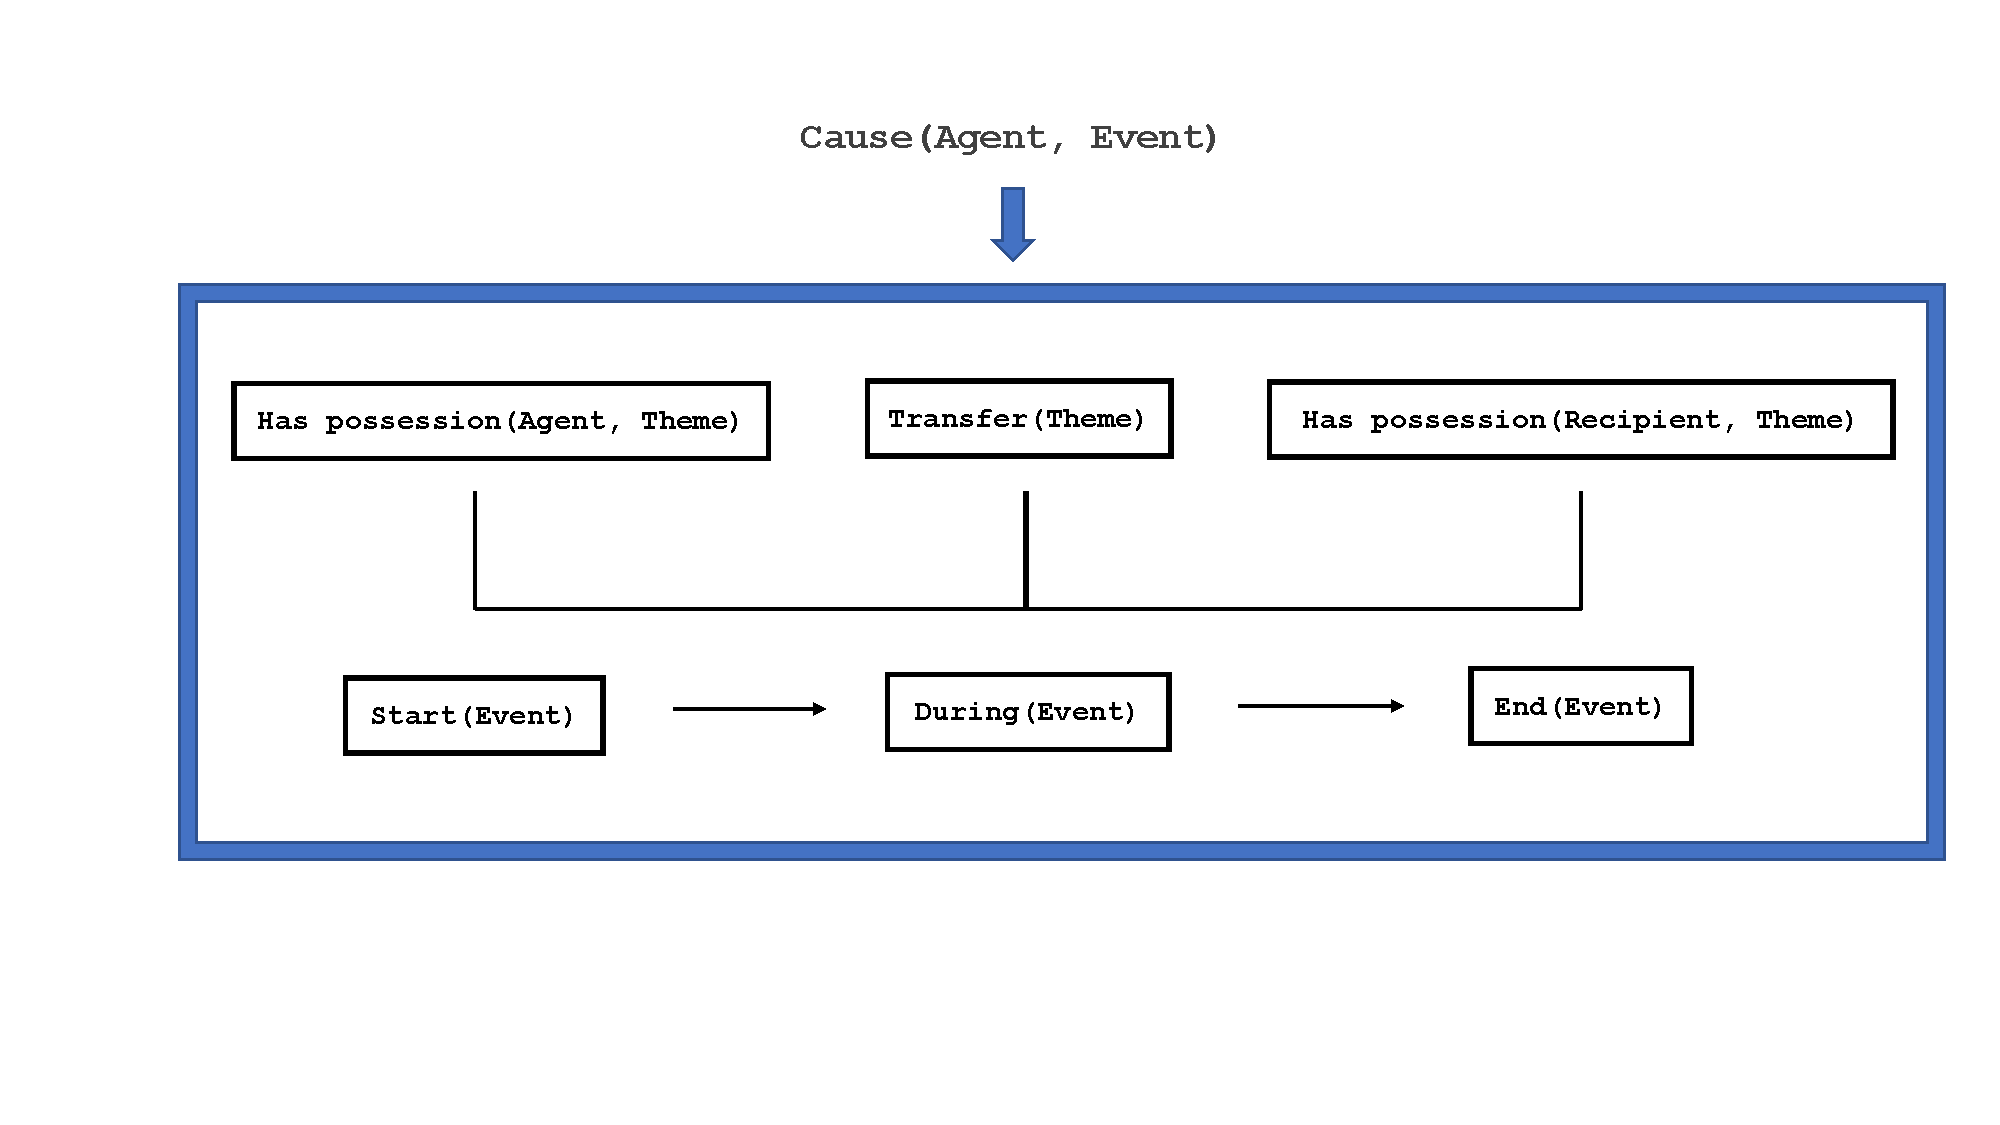
\includegraphics[width=1\textwidth, trim = {0cm 2cm 0cm 2cm},clip]{ch3/figs/semantics_give.pdf}
	\caption{prédicats sémantiques}
	\label{fig:Prédicat}
\end{figure}

Est-ce que je l'explique en détail ? Car je n'utiliserai pas du tout leur approche sémantique.
%Ainsi, dans une situation où quelqu'un prête quelque chose à quelqu'un, on retrouve un sens de causation, car l'agent qui donne un objet provoque l'existence même de l'évènement en agissant. C'est pourquoi le sens de causation domine le graphique. Puis, il y a la description de l'évènement nouvellement causé. Celui est décrit à deux niveaux simultanément. Au premier niveau, on retrouve les prédicats et leurs arguments. D'abord, le premier prédicat détient la valeur 'possession' puis ses arguments sont deux rôles thématiques (l'agent et le thème). Autrement dit, quelqu'un possède un objet. En même temps, c'est le début de l'évènement.


\subsection{Dictionnaires verbaux concurrents}

Dans la section suivante, nous faisons une revue de littérature concernant les autres dictionnaires verbaux qui existent sur le marché. Focusent généralement sur les cadres de sous-catégorisation (valence, patron de régime, structure argumentale, etc.) . Devrais-je exliquer c'est quoi ici ?

\subsubsection{WordNet}
Wordnet est une base de données lexicales traitant les verbes, noms, adjectifs et adverbes de la langue anglaise. Cette base de donnée s'organise en \emph{synset}, des ensembles de synonymes. Il ne s'agit pas de synonymes exacts, loin de là, il s'agit plutôt d'un ensemble de mots unis par des traits conceptuo-sémantiques. Ces \emph{synset} sont joints d'une définition et d'une phrase exemple. Comme VerbNet, WordNet est aussi une base de données hiérarchisée. Elle est construite via des liens d'hyperonymie et d'hyponomie entre les \emph{synsets} ce qui nous permet de naviguer dans la base de données pour visualiser dans quel concept un synset donné est inclu. Ainsi, tel que mentionné, les entrées lexicales dans ce système sont des synset et ceux-ci appartiennent à l'une des classes suivantes. S'il s'agit de verbes dénotant des actions ou des évènements, ils seront classés parmi : \emph{ motion, perception, contact, communication, competition, change, cognition, consumption, creation, emotion, perception, possession, bodily care and functions, social behavior and interactions}. S'il s'agit de verbes dénotant des états, on le retrouvera parmi les classes de type : \emph{resemble, belong, suffice,} ;  ou des classes de type : \emph{want, fail, prevent, succeed}, ou de types aspectuels comme \emph{begin} \citep{Fellbaum1998}.À l'intérieur d'une entrée, on retrouve aussi des liens de divers ordres : synonymes, antonymes, troponymes, entailment et causation.\citep{SchulerVerbnetBroadcoverageComprehensive2005}. Ce qui leur a permis de tisser une toile sémantique assez volumineuse.

À la base, WordNet a été conçu comme réseau sémantique, c'est pourquoi il contient explicitement aussi peu d'information syntaxique. La ressource fournit des définitions, des exemples et des \emph{synsets}, mais ne nous donne pas d'information sur la structure sémantique ou syntaxique des verbes. Elle est systématiquement implicite, contrairement à VerbNet qui l'explicite à l'aide de ses cadres syntaxiques. Il s'agit de la raison principale qui nous a poussé à ne pas utiliser cette ressource pour créer notre dictionnaire verbal. Nous voulions une base de données explicitant très clairement les différents actants régis par un verbe, ainsi que les prépositions sélectionnnées par celui-ci. Toutefois, notre dictionnaire a la possibilité d'être aussi mapper aux entrées de WordNet, car VerbNet a fait un mapping entre ses entrées lexicales et celles de WordNet. Chaque verbe dans VerbNet est mappé à un \emph{synset} verbal de WordNet, si c'est possible et qu'il y existe un équivalent\citep{SchulerVerbnetBroadcoverageComprehensive2005}.

manque les statistiques

\subsubsection{FrameNet}

Parallèlement au projet WordNet, s'est développé FrameNet. Le projet de Berkeley FrameNet est basé sur un corpus manuellement annoté, qui contient de l'information sur les noms, adjectifs et verbes de la langue anglaise. Dans FrameNet, les unités lexicales sont décrites en termes de \emph{frame semantics}, qu'on traduirait par la sémantique des cadres.Les semantic frames sont définis comme des représentations schématiques de situations impliquant des participants , propositions et d'autres rôles conceptuels Le but de cette ressource est d'encoder la sémantique du lexique de l'anglais dans un modèle que peuvent lire les machines \citep{BakerBerkeleyFrameNetProject1998}. Ce projet couvre la sémantique des domaines suivants : santé, chance, perception, communication, transaction, temps, espace, corps , motion, étapes de la vie, contexte sociaux, émotion et cognition. Cette base de données lexicales est composée de trois modules. D'abord, un dictionanire dont les entrées sont les unités lexicales traitées. Suivi d'un dictionnaire de \emph{frames} et complété par des exemples annotées manuellement correspondant aux \emph{frames}. Ainsi, il faut passer par le dictionnaire d'entrées lexicales, pour ensuite identifier le cadre qui lui est associé dans le dictionnaire de cadres sémantiques. Ainsi, il faut d'abord chercher dans le dictionnaire d'entrées lexicales pour ensuite trouver le ou les cadres qui lui sont associés dans le dictionnaire de cadres sémantiques. D'ailleurs, les descriptions des frames sont encodés en structures conceptuelles. Et les phrases exemples manuellement annotées sont des preuves empiriques que les \emph{frames} ont lieu d'être. Les frames décrivent la structure argumentale d'une unité lexicale. Ces arguments sont identifiés par des étiquettes similaires aux rôles thématiques. On les appelle des \emph{frame elements} et ils sont extrêmement nombreux car ils sont spécifiques aux cadrex qu'ils décrivent.En frame semantics, un frame correspond à un scénario qui implique une intéraction et des participants \citep{Shi:2005:PPT:2132047.2132058}. À noter qu'il y existe aussi une organisation hiérarchique où on a des sous-frames qui héritent de traits des frames parents. Tout comme VerbNet l'a fait avec WordNet, un mapping a été effectué entre les entrées de VerbNet et FrameNet. Cela s'est fait en deux étapes, ils ont mapper les classes de VN avec les frames de FN, puis les frames elements aux rôles thématiques \citep{Shi:2005:PPT:2132047.2132058}. Finalement, d'un point de vue pratique, FN est généralement utilisé comme \emph{semantic parser}. Des chercheurs font des parse tree syntaxique mais qui tiennent compte des participants et de leur relation avec le verbe\citep{Shi:2005:PPT:2132047.2132058}.

manque les statistiques
Expliquer pourquoi nous n'avons pas choisi FrameNet : n'explicite pas très clairement les patrons de régime. On les comprend via les phrases exemples et les frames elements, mais ce n'est pas suffisant, il y aurait beaucoup de travail à faire avant de l'implémenter dans MATE.

\subsubsection{XTAG}
Les chercheurs du projet XTAG ont construit une grammaire de la langue anglaise basé sur le formalisme de \emph{Tree Adjoining Grammar} (TAG). Cette ressource offre des descriptions syntaxiques riches des verbes en anglais. Chaque unité lexicale se fait assigner un ensemble d'arbres-TAG décrivant ses comportements syntaxiques. Les arbres reflètent la structure argumentale de ces unités lexicales. Les arbres peuvent se construire via deux opérations : substitution et adjonction. En adjoignant de nouvelles branches ou en substituant des branches, la grammaire TAG permet de rendre compte des divers phénomènes linguistiques de la langue anglaise. XTAG inclut des descriptions syntaxiques pour 33 000 items lexicaux dont 9000 verbes \citep{ResearchGroupLexicalizedTreeAdjoining2001}. XTAG organise son information syntaxique en créant des familles d'arbres. À l'intérieur de celles-ci, on distingue les arbres par des alternances syntaxiques. Ainsi, dans XTAG, Les classes verbales sont organisées de cette manière : chaque verbe dans le dictionnaire correspond à plusieurs familles d'arbres et chaque famille regorge d'arbres individuels issus de différentes transformation syntaxiques de surface pour une même structure argumentale canonique. Ainsi, on n'a pas à lister tous les arbres individuels possibles correspondant à un verbe, car celui-ci se fait assigner des familles d'arbres \citep{DoranXTAGSystemWide1994}.

Finalement, comme avec WordNet et FrameNet, Les auteurs de VerbNet ont aussi mappé leurs cadres syntaxiques aux arbres de XTAG \citep{W04-3326}.
D'ailleurs, cela leur a permis de couvrir des descriptions syntaxiques qu'ils n'avaient pas répertoriés. VerbNet couvre surtout la voix déclarative, tandis que XTAG explore toutes les transformations possibles de voix. Cependant, XTAG ne fait pas de distinctions pour les différents sens des verbes et il s'agit là d'une composante cruciale à la construction d'un bon dictionnaire en GAT. C'est pourquoi nous n'avons pas opté pour ce dictionnaire. De plus, le formalisme dans lequel les arbres sont encodés ne s'exporte pas facilement dans un format réutilisable en TST.

\subsubsection{Lexical conceptual structures-LCS}
La base de données LCS de Dorr s'est construite à partir des théories de sémantique lexicale de Jackendoff. Celui-ci argumente en faveur d'une approche de décomposition sémantique des verbes. Ceux-ci sont décrits en termes de leur structure conceptuelle lexicale\citep{DorrUseLexicalSemantics1992}. Une structure LCS est un graphe, il s'agit d'une représentation sémantique du lexique. Dans ce système, la structure syntaxique découle des primitifs sémantiques. Un graphe LCS est une représentation sémantique où il y a des noeuds dont une racine. Chaque noeud a des spécifications avec des types d'information comme : type, primitif et champ. Type ; event, state, path, manner,etc. Puis après avoir spécifier le type, on spécifie le primitif sémantique du verbe (être, aller, rester,etc.)  et les champs sont des traits qui agissent comme des restrictions sur les noeuds.Ces structures sont des représentations hiérarchiques non-linéaire composées d'une tête logique (la racine du graphe), d'un sujet logique (un seul) , d'arguments logiques et de modificateurs logiques. En ce qui concerne le traitement des verbes, la racine du graphe sera un verbe et les sujets/arguments logiques seront les participants sélectionnés par le verbe. Concrètement, ce qui décrit la sémantique des graphes est une combinaison de constituents et primitifs conceptuels et de champs sémantiques. D'abord, les constituents conceptuels appartiennent à un ensemble de catégories : chose, évènement, état, lieu, chemin, propriété, but, manière, montant, temps. Ensuite, les champs sémantiques sont des traits qui agissent comme des restrictions sélectionnelles(ex: +temp, +loc, +poss). Finalement, les primitifs conceptuels : ÊTRE, ALLER, RESTER , CAUSER, INCHOATIF, EXTENSION. Une décomposition sémantique des verbes en termes de structures lexicales conceptuelles explique leur propriété syntaxiques. Tel que Levin l'avait perçu, les propriétés sémantiques des verbes influenceront leur comportements syntaxiques. À l'intérieur de ce cadre théorique, on pense que les verbes avec des LCS similaires partagent aussi des comportement syntaxiques comme des alternances de diathèses. Ils utilisent aussi des rôles thématiques pour montrer la structure argumentale. La base de données de Dorr prend aussi la hiérarchie et se base sur les classes de Levin pour structurer son information. Dans cette base de données, les verbes sont aussi rassemblés en classes verbales. Ce qui unit les membres à une classe verbale est le partage d'une structure LCS commune. Ainsi, tous les membres d'une classe partage la même structure sémantique, mais le contenu sémantique selon chaque verbe pour satisfaire les contraintes lexicales de ceux-ci \citep{TraumGenerationLexicalConceptual2000}. 

Nous n'avons pas pris cette ressource car nos représentations sémantiques opèrent déjà la même fonction que ces graphes LCS. De plus, le caractère syntaxique de ce système ne fournit pas du tout ce que nous cherchions. Nous voulons un dictionnaire qui énumère les différents patrons de régime possibles pour un verbe donné. Toutefois, ce système a été utilisé de la même manière que nous générons du texte automatiquement en différentes langues. Cette base de données lexicales a été utilisée pour faire de la traduction automatique \citep{DorrUseLexicalSemantics1992}. Cela a été fait dans le cadre du projet UNITRAN qui traite :l'espagnol, l'anglais et l'allemand. À l'aide de représentation basées sur la LCS , ils pouvaient générer des traductions équivalentes entre les langues à partir d'une même représentation. Par la suite, les dictionnaires se chargent des spécificités de chaque langues. Notre système GenDR fonctionne aussi de cette manière.

manque les statistiques

\subsubsection{Comlex}
Comlex est une base de données lexicales développée pour l'anglais à NYU. C'est une ressource syntaxique riche, mais dont il faut débourser pour s'en servir. Les auteurs de ce système voulait  créer un dictionnaire syntaxique sur les verbes de l'anglais à des fins computationelles \citep{Grishman:1994:CSB:991886.991931}. Ils ont opté pour un système qui se voulait le plus neutre du point de vue de la théorie afin qu'il puisse être utilisé dans divers cadres de recherche. Ce dictionnaire ne traite pas uniquement que les verbes, mais c'est la partie qui nous intéresse. En ce qui concerne ceux-ci, le système décrit pour chaque verbe les compléments possibles qu'il pourrait sélectionner ainsi que les spécificités propres à certaines constructions (choix d'une préposition,etc.) Les entrées lexicales ont été manuellement ajoutées car ils ne pensaient pas que des méthodes automatiques pouvait bien rendre compte des verbes moins fréquents, et ils voulaient que leurs entrées sois dépourvues d'erreurs. Contient des descriptions syntaxiques pour 6000 verbes. 

Nous n'avons pas pris ce système car, d'abord il faut payer la license, puis nous avions lu l'évaluation que VerbNet avait menée et il en ressortait que Comlex ne distingue pas les  différents sens des verbes. Ce qui est problématique si on veut générer la phrase la plus correcte possible.

\subsubsection{A large SCF lexicon for NLP apps : Valex}
 
Valex est un projet de Korhonen, il s'agit d'un dictionnaire de cadre de sous-catégorisation (SCF) de l'anglais \citep{Korhonenlargesubcategorizationlexicon2006}. Elle a bâti son dictionnaire via des méthodes d'acquition automatiques. L'auteure vante les mérites d'une acquisition automatique et se défend en stipulant que les dictionnaires bâtis manuellement comportent naturellement plus d'erreurs. Elle pense aussi qu'ils sont plus coûteux en termes de temps et de ressource, car il faut les entretenir et les enrichir. Finalement, elle ajoute que les dictionnaires manuellement acquis comportent une faille cruciale, il leur manque de l'information statistique. Par exemple, quel cadre de sous-catégorisation est le plus utilisé pour un verbe donné et les SCF les moins fréquents.  Puisque de nombreuses applications TAL fonctionnent avec des méthodes probabilistes, la présence d'information statistique est cruciale à leur bon fonctionnement.  

Dans son article, elle explique qu'elle a utilisé le système d'acquisition de Briscoe et Caroll \citep{BriscoeSecondReleaseRASP2006} qui se base sur la méthode RASP. À partir de textes non-annotés, les SCF sont extraits grâce au système RASP. Ainsi, les données brutes provenant des corpus sont d'abord tokénisées, étiquettées, lématisées puis parsées utilisant RASP. Puis les SCF sont extraits des phrases parsées. Ainsi, chaque entrée lexicale est une combinaison d'un verbe et d'un SCF ce qui résulte en un dictionnaire de base. Finalement, il est filtré car, puisque c'est une méthode automatique, le système déduit des SCF qui n'en sont pas. Il faut donc les retirer du dictionnaire. D'ailleurs, ces systèmes se retrouvent avec des problèmes de rappel. Certains SCF ne seront pas extraits puisque le système ne les reconnaîtra pas comme des SCF. Ils utilisent des dictionnaires construits manuellement pour trouver ces SCF manquants.

Dans Valex, une entrée lexicale comprend entre autre : la combinaison d'un verbe et d'un SCF, la syntaxe des arguments, la fréquence d'utilisation du SCF. Bien que ce système aurait été potentiellement bon, nous avons préféré nous tourner vers VerbNet. D'abord, ce dictionnaire ne différencie pas les sens des verbes, de plus, l'architecture du logicielle ne nous permet pas de tirer parti du principe d'héritage des traits. Contrairement à VerbNet qui le permet, d'autant plus que ça permet de réduire la quantité d'information dans notre dictionnaire. Finalement, comme notre système fonctionne avec des règles de grammaire et que ce n'est pas un générateur de texte basé sur des méthodes stochastiques, l'apport d'informations statistiques que Valex offre ne nous était pas utile pour l'instant.

statistiques : coverage

\subsubsection{LexSchem}
LexSchem est un dictionnaire de verbe pour le français créé par Messiant. Il jusitifiait la valeur de son projet en disant que  que l'information la plus utile qu'un dictionnaire peut offrir sont les cadres de sous-catégorisation des verbes \citep{MESSIANT08.142}. Ces \emph{subcategorization frame} (SCF) capturent, au niveau syntaxique, les différentes combinaisons d'arguments qu'un prédicat lie. Messiant ajoute que comme les verbes sont au centre des énoncés, un dictionnaire qui se concentre sur les cadres de sous-catégorisation peut être très bénéfiques à des applications TAL.  Nous avons vu jusqu'à maintenant qu'ils peuvent être utilisés pour le parsing et la traduction automatique par exemple. Toutefois, suivant les pas de Korhonen \citep{Korhonenlargesubcategorizationlexicon2006}, Messiant a bâti un dictionnaire de SCF pour le français via une acquisition automatique. Il se justifie en disant que cette technique a déjà fait ses preuves dans des applications réelles malgré le fait qu'elle n'est pas aussi précise et détaillée qu'une approche manuelle. Mais elle est beaucoup moins coûteuse en termes de temps et de ressource. De plus, une approche automatisée permet d'extraire de l'information qui pourrait s'avérer très utile pour des applications TAL. Notamment, les statistiques et la fréquence d'utilisation d'un SCF.  Son dictionnaire a été acquis à partir de corpus non-annoté. Par la suite,les SCF acquis automatiquement sont incorporés dans lexSchem. Voici la démarche qu'il utilisa, d'abord ils prennent des données brutes, puis il étiquette et lemmatise les mots  pour ensuite parser le tout. Après il ne reste qu'à en extraire les SCF. Dans LexSchem, Les entrées lexicales sont composées essentiellement de : L'unité lexicale, ses cadres de sous-catégorisation et des phrases exemples tirées de corpus ainsi que la fréquence d'utilisation du SCF.

Ce que nous retenons de ce système, c'est qu'il pourrait être utile dans un avenir où nous voulions extraire VerbeNet qui est une version francophone de VerbNet. Nous pourrions ainsi complémenter la ressource francophone par une autre ressource franchophone. De plus, tel que VerbNet l'a fait, LexSchem construit ses entrées lexicales en misant sur les cadres de sous-catégorisation. Nous pensons aussi qu'un dictionnaire verbal en TAL devrait surtout incorporer ces données, ce qui nous intéresse sont les cadres de sous-catégorisation, car ceux-ci sont la partie la plus dure à traiter en TAL.

statistiques:

\subsubsection{VDE-Valency dictionary of English}
Le VDE est un dictionnaire de valence tout comme les dictionnaires précédents qui liste la manière dont un verbe peut se combiner avec ses arguments \citep{HerbstValencyDictionaryEnglish2004}. Le VDE contient les valences de 511 verbes (il traite aussi les noms et les adjectifs). Dans ce dictionnaire, chaque entrée décrit une valence possible pour un verbe accompagné d'un exemple provenant de la \emph{Bank of English}. Lors de sa création, le VDE n'était pas destiné à des applications TAL, mais les auteurs se sont rapidement rendus compte que ça pourrait intéresser des linguistes computationnels. Ainsi est né le \emph{Erlangen Valency Pattern Bank} \citep{faucris.1039365}, un outil de TAL qui liste les patrons de valence identifié par le VDE.  Dans le VDE, les 511 verbes qui y figurent ont été choisis sur la base qu'ils sont fréquents dans la langue anglaise, qu'ils démontrent des propriétés complexes et qu'ils sont utiles pour des apprenants de l'anglais. Les patrons de valence qu'on retrouve dans le VDE proviennent d'une étude de corpus fait sur le COBUILD. Les patrons y sont décrits en termes de syntaxe de surface.  Leur dictionnaire est réparti en deux où d'un côté on a la liste des 511 verbes et les patrons de valence leur étant associés, puis dans un autre dictionnaire les patrons de valence de la langue anglaise. Il s'agit aussi d'un système qui distingue les différents sens que peuvent prendre les verbes. 

Bref, il s'agit d'un dictionnaire qui couvre de verbes, mais les plus fréquents. Toutefois, il s'agit d'un travail manuel, donc on s'attend à ce qu'il ne comporte pas beaucoup d'erreurs, et on pourrait ainsi en extraire une partie pour complémenter le dictionnaire de VerbNet si tel est le besoin.

%Thomas Herbst and Peter Uhrig. 2009. Erlangen Valency Pattern Bank – a corpus-based research tool for work on valency and argument structure constructions. Website. http://www.patternbank.uni-erlangen.de

\subsubsection{Dicovalence}
Le Dicovalence est un dictionnaire de valence pour la langue française. Une entrée lexicale dans ce dictionnaire correspond à la combinaison d'un verbe, d'un cadre valenciel et d'un exemple. Comme il y a 3700 verbes traités et que la plupart des verbes comptent plus d'un cadre valenciel, il y a plus de 8000 entrées lexicales dans ce dictionnaire. Les informations à l'intérieur des cadres valenciels sont décrites par l'approche pronominale en syntaxe \citep{11403/dicovalence/v1}. Dans leur système, ce que plusieurs appellent des participants, des actants ou des arguments, sont appelés des paradigmes. Le Dicovalence a aussi été créé dans une optique de TAL et d'enseignement de la langue. Contrairement à des systèmes comme FrameNet, ou VerbNet, ils identifient leurs arguments en les numérotant. Le paradigme p0 étant souvent le sujet, le p1 étant l'objet direct, le p2 étant l'objet indirect et tous les autres étant des obliques. Ce dictionnaire contient beaucoup d'information utile autre que les cadres valenciels. Il y a  : des phrases exemples, des traductions du verbe en anglais et en allemand, des restrictions sélectionnelles sur les paradigmes, le type d'auxiliaire (avoir/être) et les constructions passives.

Nous n'utiliserons pas ce système puisque nous traitons l'anglais, mais le survol de ce système nous confirme que VerbNet était un bon choix, car les entrées importantes sont souvent les mêmes. Les cadres syntaxiques, les phrases exemples. Toutefois, nous pourrions nous en servir pour compléter l'implémentation de VerbeNet français dans notre système pour une génération multilingue.

%https://repository.ortolang.fr/api/content/dicovalence/1/documentation/DicovalenceManuel_v20_100625.pdf
%Karel van den Eynde and Piet Mertens. 2006. Le dictionnaire de valence DICOVALENCE : manuel d’utilisation. http://bach.arts.kuleuven.be/dicovalence/manuel 061117.pdf.

\subsection {Utilisation de VerbNet dans des applications NLP}

VerbNet a été utilisé dans un nombre impressionnant de travaux de recherche. Ce qui en témoigne de son efficacité et de sa réputation. Voici notamment quelques projets de recherche où les chercheurs se sont servis de cette base de données lexicales pour effectuer leurs travaux.

\subsubsection{Automatically building conceptual graphs using VerbNet and WordNet}
\citep{HensmanAutomaticallyBuildingConceptual2004}

\subsubsection{Putting Pieces Together: Combining FrameNet, VerbNet and WordNet for Robust Semantic Parsing}
\citep{Shi:2005:PPT:2132047.2132058}

\subsubsection{Question Answering with Lexical Chains Propagating Verb Arguments}
\citep{Novischi:2006:QAL:1220175.1220288}

\subsubsection{A question answering system based on VerbNet frames}
\citep{questionansweringsystem}

\subsubsection{A supervised algorithm for verb desambiguasation into VerbNet classes}
\citep{AbendSupervisedAlgorithmVerb2008}

\subsubsection{Semantic classifications for detection of verbs metaphor}
\citep{DBLP:conf/acl/KlebanovLGSF16}

\subsubsection{VerbNet class assignment as a wsd task}
\citep{BrownVerbNetClassAssignment2011}

\subsubsection{Multilingual NLG within abstractive generation}
\citep{GalanisGeneratingMultilingualDescriptions2007}

\subsection{Pourquoi on n'a pas utilisé les rôles thématiques et les prédicats sémantiques}

\citep{mel2012semantics}
Parler de ça dans la section python où on crée les patrons de régime, ça s'y prêtre plus.
p.210 dans le livre Melcuk
on pourrait garder les rôles pis les mettre dans MATE aussi

\subsection{Pourquoi avoir choisi VerbNet ?}

Nous avons choisi VerbNet car :

coverage, architecture, désambiguisation, descriptions syntaxiques facilement exportable, traitement en Python très accessible, existe bcp de VerbNet dans d'autres langues, et comme notre système se veut multilingue, c'est un premier pas pour facilement exporter les autres langues par la suite. Déjà utilisé pour bcp de tâches NLP, dont NLG.

D'autres ont aussi utilisé VerbNet pour ce genre de tâche, notamment : jonathan pfeil et Offer Biller

le tutoriel : ESCW tuto RelExtra v1	

Wanner et Mille avait aussi démontré un intérêt vers VerbNet en 2016 pour ce genre de tâche.



%%%%%%%%%%%%%%%%%%%%%%%%%%%%%%%%%%%%%%%%%%%%%
% ---------  P Y T H O N  ---------
%%%%%%%%%%%%%%%%%%%%%%%%%%%%%%%%%%%%%%%%%%%%

\section{Python}

À l'aide du module \emph{xml.etree.cElementTree} nous avons pu faire des opérations sur l'ensemble des données de VerbNet qui sont encodées dans des fichiers XML. Le module Etree nous permet de naviguer dans les fichiers XML de VerbNet puis de manipuler et d'extraire les données qui nous intéresse. Après avoir manipulé et extrait les données intéressantes, nous les avons compilées dans des dictionnaires. Ceux-ci seront utilisés par notre système MATE pour générer du texte automatiquement. Par la suite, nous avons aussi utilisé Python et le module Etree pour extraire les phrases exemples qui accompagent chaque patron de régime couvert par la ressource lexicale. Dans le but de créer des structures sémantiques qui nous serviront d'input pour générer en syntaxe de surface la phrase exemple et ainsi vérifier si MATE est capable de générer les phrases exemples.

Nous voulions donc créer des documents DICT qui seraient l'information lexicale de notre système de GAT. Il est d'abord important de dire dans les grandes lignes comment notre système MATE fonctionne. Ainsi, notre système prend en input une représentation sémantique d'un énoncé, puis fait appel à des dictionnaires et des règles de grammaire pour générer en output une représentation syntaxique de surface de l'énoncé. Les unités lexicales s'encodent d'une certaine manière dans MATE et nous voulions créer nos dictionnaires à l'image des contraintes données par le système MATE. Nous avons donc codé la manipualtion et l'extraction des données en fonction de la manière dont le lexique est encodé dans MATE.

\subsection{Création du dictionnaire de verbes: lexicon.dict}

La première étape de notre projet consistait à créer le dictionnaire verbal. Bien que le dictionnaire final comporte 6393 entrées lexicales verbales, cette partie de code nous permettait de créer la base de notre système. Il serait important de décrire dans les grandes lignes à quoi ressemble le dictionnaire pour mieux expliquer pourquoi nous l'avons extrait de cette manière. Ainsi MATE possède la caractéristique d'héritage des traits. Donc, en ce qui concerne les verbes, nous avons architecturé la chose de cette manière. Il existe une classe des verbes qui ont les traits suivants : une dpos=V et une spos=verb.

\begin{lstlisting}[language=XML]
verb {
  dpos = V
  spos = verb
}
\end{lstlisting}

Ensuite, les 278 classes verbales de VerbNet pointent vers la classe verb, donc les classes héritent de ces deux traits. Ce qui fait en sorte qu'on n'a pas a répété dans chaque entrée de classe verbale les traits dpos et spos. 

\begin{lstlisting}[language=XML]
"absorb-39.8": verb {
  gp = { id=NP_V_NP                        dia=12 } // Cotton absorbs water.
  gp = { id=NP_V_NP_PP_from_source         dia=123 } // Cattle take in nutrients from their feed.
}
\end{lstlisting}

Ensuite, chaque membre de chaque classe verbale pointe vers la classe ou la sous-classe qui le représente ce qui fait en sorte qu'il hérite de tous les traits de la classe(sous-classe) vers laquelle il pointe. Par exemple : absorb, ingest, take in vont tous trois hériter des traits de l'entrée "absorb-39.8" qui est la classe verbale. C'est de cette manière que notre dictionnaire passe de 278 entrées lexicales à 6393. Car, les verbes de la langue anglaise ont été classés dans des classes verbales et nous les intégront à notre dictionnaire en gardant la même architecture que VerbNet avait pensé (basé sur les travaux de Levin).

\begin{lstlisting}[language=XML]
absorb : "absorb-39.8"
take_in : "absorb-39.8"
ingest_1 : "absorb-39.8"
\end{lstlisting}

\subsubsection{Création du dictionnaire initial contenant les 278 classes verbales comme entrées lexicales}

\begin{lstlisting}[language=Python, caption = code pour lexicon.dict]
# BLOC 1
def supers(t, i):
    ID = t.get('ID')
    sc = {ID:i}
    subclasses = t.findall('SUBCLASSES/VNSUBCLASS')
    if len(subclasses) > 0:
        for sub in subclasses:
            sc = {**sc, **supers(sub, ID)}
    return sc
		
# BLOC 2
def treeframes(t):
    ID = t.get('ID')
    z = []
    for frame in t.findall('FRAMES/FRAME'):
        description = re.sub(r"\s*[\s\.\-\ +\\\/\(\)]\s*", '_', 
        frame.find('DESCRIPTION').get('primary'))
        if description in exclude:
            continue
        description = re.sub('PP', 'PP_{}', description)
        preps = [p.get('value') or 
                p.find('SELRESTRS/SELRESTR').get('type').upper() 
                for p in frame.findall('SYNTAX/PREP')+frame.findall('SYNTAX/LEX')]
        preps = [sorted(p.split()) for p in preps]     
        examples = [e.text for e in frame.findall('EXAMPLES/EXAMPLE')]
        if len(preps)==1:
            description = description.format('_'.join(preps[0]))
        elif len(preps)==2:
            description = description.format('_'.join(preps[0]),
                                             '_'.join(preps[1]))
        elif len(preps)==3:
            description = description.format('_'.join(preps[0]), 
                                             '_'.join(preps[1]), 
                                             '_'.join(preps[2]))
        z.append((description, examples))
        
    subclasses = t.findall('SUBCLASSES/VNSUBCLASS')
    subframes = [treeframes(subclass) for subclass in subclasses]
    subframes = sum(subframes, []) # flatten list of lists
    return [(ID, z)] + subframes
		
# BLOC 3
with open('lexicon.dict','w') as f:
    f.write('lexicon {\n')
    for file in [f for f in os.listdir('verbnet') if f[-4:] == '.xml']:
        root = ET.parse('verbnet/'+file).getroot()       
        d = dict(treeframes(root))
        sc = supers(root, 'verb')
        for c in d.keys():
            f.write('"'+c+'"')
            if sc[c] == 'verb':
                f.write(': ' +sc[c] + ' {')
            else :
                f.write(': ' +'"'+sc[c]+'"' + ' {')
            [f.write('\n  gp = { id=' + gp[0] + (max(len(gp[0]), 30)-len(gp[0]))
                     *' ' + ' dia=x } // ' + ' '.join(gp[1])) for gp in d[c]]
            f.write('\n}\n')
    f.write('\n}')
\end{lstlisting}

Ce script sert à :

On l'a découpé en trois blocs pour faciliter l'explication.

Expliquons d'abord le premier Bloc 
Expliquos ensuite le deuxième Bloc
Expliquons finalement le troisième Bloc

Faire du plus général au plus précis, puis ensuite bloc par bloc
-Décrire ce que je veux que la fonction fasse dans les grandes lignes
-Expliquer un peu plus concrètement ce que je veux que ça fasse
-Expliciter mon code encore plus précisément
-Mettre en commentaire la nature des variables

(Peut-être rajouter les numéros de lignes, ce sera utile pour faire référence à des lignes de code)
Ce premier script Python se découpe en trois blocs. Les deux premiers blocs sont des fonctions que nous définissons pour ensuite les utiliser dans le BLOC 3 qui nous permettra d'écrire le dictionnaire initial.  Ainsi, pour une meilleure compréhension du script complet, nous décrirons les blocs 1 et 2 pour expliquer ce que les fonctions font, ensuite nous décrirons le bloc 3 car l'usage des fonctions sera maintenant clair.

Commençons par la première fonction supers. La fonction prend 2 arguments : t et i. Si vous regardez le bloc 3, dans la section sc, on voit que supers prend les arguments (root, 'verb'). Ces deux arguments sont les suivants : root donne accès à l'arbre XML et 'verb' est fait pour que chaque classe verbale pointe vers la catégorie verbe. Pour en hériter les traits dpos=V et spos=verb.  On va chercher le trait ID dans l'un des deux arguments (l'argument arbre donc montré dans listing le trait ID dans le XML). Ensuite on crée un dictionnaire s'appelant sc dont la clé est le ID et la valeur est i. Puis on instancie une variable subclasses qui contient les racines de chaque sous-classes dans les documents XML (montrer avec listings à quoi ça ressemble dans le document XML). Puis ensuite, pour chaque élément dans sous-classe (si élément il y a) on lui passe la fonction supers et on va chercher son identifiant car en lui repassant la fonction, on retourne a sub.get('ID') donc on va chercher le ID qui se retrouve dans la partie sous-classe de l'arbre de la classe verbale et on met à jour le dictionnaire sc en y ajoutant les identifiants des sous-classes (les clés) qui pointeront vers l'identifiant de la classe qui le gouverne, car le deuxième argument de supers est une chaîne de caractère, dans ce cas, la chaîne ID qu'on avait pu chercher plus tôt dans la fonction. Cela est fait dans le but de construire: sous-classe : classe (donc la sous-classe hérite des traits de sa classe) grâce au mécanisme d'héritage de MATE, et tel que VerbNet le mentionne, chaque sous-classe hérite des traits donnés par la classe qui la domine. 

Maintenant, passons à la seconde fonction treeframe. Cette fonction prend un argument. On va aller chercher ID. Puis on initialise une liste z. Pour tous les frames qu'on retrouve dans l'arbre en question, on va chercher la description primaire du frame. On va ensuite se servir des expressions régulières pour uniformiser les descriptions à notre bon vouloir. Parallèlement, nous avons aussi créé une liste s'appelant exclude qui contient toutes les descriptions que nous voulons exclure de notre système et si une description dans un frame se retrouve aussi dans exclude, alors on n'y touche pas et elle ne sera pas modifiée ni ajoutée à la liste description. Ensuite, on modifie encore le nom des descriptions car nous ferons une opération par la suite. Donc, on modifie toutes les descriptions qui contiennent PP pour qu'elles ressemblent à 


%Nous avons donc utilisé VerbNet de mieux que nous le pouvions. Ainsi, les descriptions des FRAMES SYNTACTIC étaient "accurates" et allait nous donner les brèves descriptions des patrons de régime que nous ajouterons à notre lexiconCar, nous pensions au départ que nous pourrions tout prendre de verbnet pour créer notre lexicon.  Nous voulions chercher les descriptions des patrons de régime ainsi que l'information sous SYNTAX sous FRAME pour ainsi créer les patrons de régime en soi en les traduisant dans notre langage (TST). Toutefois, leur manière d'encore les patrons de régime ne correpond pas à la notre sur beaucoup trop d'aspect. Nous le verrons plus tard, il y a de la redondance à certains moments et notre théorie rend mieux compte des patrons de régime. Mais pour l'instant, ce qui est important de noter c'est que nous notons les patrons de régime en attribuant des actants I et des noms de relation pour signifier que est le rôle de cet actant lors du passage de la sémantique à la syntaxe. VerbNet ne fait pas cela de la même manière que nous. Ils ont aussi un volet sémantique, mais qui ne se branche pas à notre modèle théorique. Nous voulions donc nous inspirer quand même de leur méthode pour nos patrons de régime, mais le fait qu'ils utilisent les rôles thématiques nous posait problème. Il était difficile d'associer un rôle thématique à un actant syntaxique (bien que nous ayons tenté [montrer le graphique de F.L]). Donc, nous en sommes venus à la conclusion qu'il nous faudrait créer les patrons de régime en Python pour ensuite les exporter dans un format adéquat pour MATE. Pour ce faire, nous devions utilisé les descriptions des patrons de régime qui se retrouve dans \emph{ VerbNet} et à partir de la description, créer une fonction qui nous permettrait de générer rapidement des patrons de régime adéquat pour MATE en ayant simplement à remplir les trous. 

%Pour extraire les descriptions des patrons de régime nous avons utilisé deux fonctions. D'abord la fonction \emph{treeframe} qui s'occupe de récupérer la description de chaque frame syntaxique à travers tout VN. Nous passons à travers tous les frames existant dans les XML de VN. Autant dans les classes que les sous-classes. Toutefois, cette fonction ne fait pas que récupérer la description du syntactic frame de VN et nous la recrache tel quel. Nous faisons quelques opérations sur les descriptions que nous extrayons. Notamment, nous remplaçons tout espace,tiret, point,barre oblique, paranthèses qui pourraient se trouver dans les descriptions par des {\_} à l'aide d'expressions régulières. Puis, nous retirons certaines descriptions de gp à cause de leur caractèrere problématique à encoder(pour des raisons théoriques, logiques -- à expliquer ailleurs).Puis une fois qu'un clean up a été fait des descriptions et que nous avons uniquement celles que nous voulions, nous procédons à une seconde étape de raffinement des descriptions. Nous utiliserons une seconde fois une expression régulière pour trouver tous les occurrences de PP car nous ajouterons les prépositions impliquées dans les PP comme tel. Pour ce faire, nous faisons un search de tous les prépositions existant dans les patrons de régime de verbnet(et non dans la description, c'est là que les patrons de régime de VN nous ont été utiles) et nous mettons les prépositions que nous soutirons des gp directement dans le nom de la description des gp à la suite du mot PP à chaque fois qu'on retrouve le mot PP dans une description. On obtient ainsi les descriptions nettoyées de celle qu'on ne veut pas, avec uniquement des underscore pour séparer les syntagmes puis les prépositions (lorsqu'il y a lieu) dans les noms des descriptions de gp.

%Puis, une fois que nous faisions ces opérations sur les classes de VerbNet, nous avons scripté une méthode pour que la fonction s'applique aussi aux sous-classes.

%Par la suite, nous avons créé une fonction \emph{super} afin que la création du lexicon s'agence bien avec la manière que MATE fonctionne. Cette fonction nous permet d'utiliser le mécanisme d'héritage qui existe dans MATE. Ainsi, on peut renvoyer une sous-classe à la classe(ou sous-classe) qui la domine. De plus, cette fonction limite le nombre de descriptions de gp. VerbNet a aussi ce mécanisme d'intégrer autrement. Ainsi, si une classe X a 10 descriptions et qu'une sous-classe Y en a 5, mais que les 10 descriptions de la classe s'appliquent aussi à la sous-classe, on n'aura pas 15 descriptions mais juste 5 dans le sous-classe, car le mécanisme d'héritage s'occupe de faire ça. On a aussi programmé la création den notre lexicon pour que si il n'y a pas de sous-classes, que la classe hérite de la classe verb afin d'avoir les attributs de base de cette classe (la dpos, la spos, voir MATE). De cette manière, tous les classes héritent de la classe verb si on remonte aux classes mères, ainsi, on n'a pas besoin de préciser à chaque fois la dpos/spos.

%Puis finalement, nous  utilisons la fonction write qui écrit le tout dans un fichier .dict. Nous loopons à travers tous les fichiers compris dans le dossier VN. Puis nous allons chercher les keys et values du dictionnaire créé à l'aide de la fonction treeframe et du dictionnaire super.(À revoir)

%Nous avons aussi pris la peine d'extraire les exemples pour chaque description car il s'agit d'une information utile pour voir dans quel contexte s'utilise ce patron de régime. Et c'est une information pertinente à avoir dans un dictionnaire, donc nous l'ajouterons à notre lexicon pour notre système de GAT. Pour ce faire, nos opérons de la même manière que pour les descriptions de gp dans le sens où nous faisons l'extractiond exemples en passant par les feuilles XML et le module d'extraction xml.etree. Pour chaque frame, nous passons la fonction à l'entièreté de VN et nous nous arrêtons à la balise EXAMPLES puis à tout texte se trouvant dans cette balise. Nous avons voulu extirper les exemples alongside des descriptions car c'est de l'information pertinente à avoir dans un dictionnaire.

\subsubsection{Extraction des 6393 membres des classes verbales pour enrichir le dictionnaire lexicon.dict}

\begin{lstlisting}[language=Python, caption = code pour ajouter des lexèmes à lexicon.dict]
def treemember(t):
    ID = t.get('ID')
    members = [m.get('name') for m in t.findall('MEMBERS/MEMBER')]
    subclasses = t.findall('SUBCLASSES/VNSUBCLASS')
    submembers = []
    if len(subclasses) > 0:
        for sub in subclasses:
            submembers = submembers + treemember(sub)
    return [(ID, members )] + submembers

files = [f for f in os.listdir('verbnet') if f[-4:] == '.xml']

members = dict(sum([treemember(ET.parse('verbnet/'+file).getroot()) for file in files], [])) # ici on a classe : [membre,...]
values = sum(list(members.values()), []) # ici c'est uniquement les membres, sans infos sur leur classe
dups = {m:[ID for ID in members.keys() if m in members[ID]] for m in values if values.count(m)>1}
unique_member = {m:ID for ID in members.keys() for m in values if m in members[ID] and values.count(m)==1}
lexemes = {d[0]+'_'+str(n+1):d[1][n] for d in dups.items() for n in range(len(d[1]))}

# Ici, je fusionne les dictionnaires ensemble
unified_dict = {**unique_member, **lexemes}

with open('members.dict','w') as f:
    f.write('members {\n')
    for key in sorted(unified_dict.keys()):
        f.write(key)
        f.write(' : '),
        f.write('"'+str(unified_dict[key])+'"')
        f.write('\n')
    f.write('\n}\n')

\end{lstlisting}

\subsection{Création du gpcon}

\begin{lstlisting}[language=Python, caption = code pour gpcon.dict]
def roman(n):
    return ['I', 'II', 'III', 'IV', 'V', 'VI'][n-1]
		
def gp(name, real_actant):
    s = name + ' {\n'
    i=0
    for actant in real_actant:
        i = i+1
        if type(actant) == list:
            for y in actant:
                s = s + "   " + roman(i) + "={" + y + "}\n"
        else:
            s = s + "   " + roman(i) + "={" + actant + "}\n"
    s = s + '}\n'
    return s


#SUBJECTIVE
subj = 'rel=subjective dpos=N'

#DIRECT OBJECTIVE
dir_N = 'rel=dir_objective dpos=N'
dir_V_ING = 'rel=dir_objective dpos=V finiteness=GER'
dir_V_INF = 'rel=dir_objective dpos=V finiteness=INF'

#INDIRECT OBJECTIVE
to_N = 'rel=indir_objective dpos=N prep=to'
indir_N = 'rel = indir_objective dpos = N'

#OBLIQUE
on_V = 'rel=oblique dpos=V prep=on'
to_obl_N = 'rel=oblique dpos=N prep=to' 
for_obl_N = 'rel=oblique dpos=N prep=for'
as_N =  'rel=oblique dpos=N prep=as'
against_N = 'rel=oblique dpos=N prep=against'
at_N = 'rel=oblique dpos=N prep=at'

# LOC

locab = 'rel=oblique dpos=N prep=locab'
locad = 'rel=oblique dpos=N prep=locad'
locin = 'rel=oblique dpos=N prep=locin'

descriptions = {
'NP_agent_V' : [subj],
'NP_agent_V_NP' : [subj, dir_N],
'NP_asset_V_NP_PP_from_out_of' : [subj, dir_N, [from_N, out_of_N]],
'NP_attribute_V' : [subj],
'NP_attribute_V_NP_extent' : [subj, dir_N],
'NP_attribute_V_PP_by_extent' : [subj,by_N],
'NP_cause_V_NP' : [subj, dir_N ],
'NP_instrument_V_NP' : [subj, dir_N],
'NP_location_V' : [subj],
'NP_location_V_NP_theme' : [subj,dir_N],
'NP_location_V_PP_with_agent' : [subj, with_N],
'NP_location_V_PP_with_theme' : [subj, with_N],
'NP_material_V_NP' : [subj,dir_N],
'NP_material_V_PP_into_product' : [subj, into_N],

# CREATION DU GPCON
with open('gpcon.dict','w') as f:
    f.write('gpcon {\n')
    for d in descriptions.keys():
        f.write(gp(d, descriptions[d]))
    f.write('}')

\end{lstlisting}

Rajouter aussi en lstlistings les résultats qui sont des documents .dict (à la fin de l'explication)

Soit le mentionner ici, ou ailleurs, mais il a fallu faire un dictionnaire de patron de régime. D'abord, parce qu'on s'est rendu compte que du à toute l'information qu'on allait chercher et la différence dans le type d'information, on a jugé bon de créer un second dictionnaire qui ne contiendrait que les gps, autrement dit un gpcon. Celui l'information sur les patrons de régime (les actants syntaxiques). Il existe x nombre de gps répertoriés. Nous les avons trouvé en faisant un ensemble à partir de tous les descriptions que nous avons obtenus avec le script précédent. Une fois que nous avons l'ensemble des gps différents. Il nous fallait les créer, car tel que mentionné, nous ne pouvions pas extraire les gps de VerbNet dû à une différence trop grande (cadre théorique et application). Notre système de GAT fonctionne avec la théorie Sens-Texte et nous pensons que c'est la théorie qui s'y prête le plus pour faire ce type d'opérations et qui tient le mieux compte de la manière dont le langage fonctionne. Ainsi, nous avons créer le gpcon à partir de Python car un bon nombre d'opérations peuvent être automatisés (éviter les fautes, et c'est plus transparent). Pour la création du gpcon, notre dictionnaire en Python ressemblait à ça. Nos keys() étaient la description du gp et les valeurs étaient les actants syntaxiques impliqués dans ce gp (avec de l'information sur les actants syntaxiques nécessitant une préposition à réaliser). Selon l'ordre dans lequel figure nos objets dans la liste qui est ce qu'on retrouve dans values(), notre fonction va assigner le bon actant syntaxique(I, II, III, etc.) ainsi, cette partie est automatisée grâce à cette fonction. Après, pour l'objet "subj" on va lui assigner une string 'rel=subjective dpos=N' ce qui est encodé dans une autre cellule. Ainsi à chaque fois qu'un gp a  un subj, on n'a pas à écrire ce que subj contient. Alors pour l'objet subj, on aura I et 'rel=subjective dpos=N'. C'est l'union de la fonction gp et de la fonction roman qui nous permettent d'assigner les bons actants syntaxiques aux objets dans la liste qui représente les values dans mon dictionnaire de gpcon.

\subsection{Scripts pour faire les tests}

\subsubsection{Extraction des exemples}

\begin{lstlisting}[language=Python, caption = code pour créer phrases.txt]
def treeframes(t):
    z = []
    for frame in t.findall('FRAMES/FRAME'):
        description = re.sub(r"\s*[\s\.\-\ +\\\/\(\)]\s*", '_', frame.find('DESCRIPTION').get('primary'))
        if description in exclude:
            continue    
        examples = [e.text for e in frame.findall('EXAMPLES/EXAMPLE')]
        z =  z + examples 
    subclasses = t.findall('SUBCLASSES/VNSUBCLASS')
    subframes = [treeframes(subclass) for subclass in subclasses]
    subframes = sum(subframes, []) # flatten list of lists
    return z + subframes

liste=[]
with open('phrases.txt','w') as f:
    for file in [f for f in os.listdir('verbnet') if f[-4:] == '.xml']:
        root = ET.parse('verbnet/'+file).getroot()       
        d = (treeframes(root))
        final_liste = liste + d
        [f.write(x+'\n') for x in final_liste]

\end{lstlisting}

\subsubsection{Création des structures qui serviront de tests}

Dans la figure ci-bas, on explique comment on a créer les documents .str qui serviront d'input à notre système MATE qui prend ce genre de document en entrée.

\begin{lstlisting}[language=Python, caption = code pour créer des structures .str]
phrases = open('phrases.txt','r')

with open('structures.str','w') as f:
    for(i,p) in enumerate(phrases):
        with open('s'+str(i)+'.str','w') as g:
            structure = 'structure Sem S'+str(i)+'{\n S {text="'+p.strip()+'"\n\n main-> \n }\n}'
            f.write(structure)
            g.write(structure)
\end{lstlisting}
